\subsubsection{Templates}
\label{sec:3_WC_Templates}

Das folgende Kapitel basiert ausschließlich auf der Spezifikation von Templates des W3C \citereset \autocite[siehe][]{Weinstein.2013} und auf dem Artikel \glqq HTML's new Template Tag\grqq\ \citereset \autocite[siehe][]{BidelmanTemplate.2013}.

Laut W3C sind Templates
\begin{quote}
\glqq
  a method for declaring inert DOM subtress in HTML and manipulating them to instantiate document fragments with identical contents.
\grqq
\end{quote}
Somit sind Templates eine Methode um inaktive DOM-Unterstruktur in HTML zu deklarieren und zu manipulieren, um so sämtliche identische Dokumentfragmente mit identischem Inhalt zu instanziieren.

In Web-Applikationen wird oft die gleiche Unterstruktur von Elementen wiederverwendet, mit dem passenden Inhalt gefüllt und zum Dokument hinzugefügt. Ein Beispiel in disem Kontext wäre eine Liste von Artikel, die mit mehreren \lstinline|<li>| -Tags in das Dokument eingefügt werden. Des Weiteren kann jeder \lstinline|<li>|-Tag weitere Elemente, wie beispielsweise einen Link, ein Bild, einen Paragraphen, etc., enthalten. Derzeit bot HTML keine native Möglichkeit an, eine solche Aufgabenstellung zu lösen.

Folgend wird eine Liste von Autos mit Hilfe eines Templates erstellt:
\begin{lstlisting}[language=HTML, caption={Web-Components Template-Standard}, label={lst:3_Templates}, escapeinside={@}{@}]
<template id="carTemplate">
  <li>
    <span class="carBrand"></span>
    <span class="carName"></span>
  </li>
</template>
\end{lstlisting}

Ein Template, wie das aus Code-Beispiel \ref{lst:3_Templates} auf Seite \pageref{lst:3_Templates}, kann sowohl im \lstinline|<head>|- als auch im \lstinline|<body>| definiert werden. Das Template, inklusive Subtree, ist inaktiv. Wenn sich ein \lstinline|<img>|-Tag mit einer validen Quelle in diesem Template befinden würde, würde der Browser dieses Bild nicht laden. Darüber hinaus ist es nicht möglich ein Element des Templates via JavaScript zu selektieren, wie in Code-Beispiel \ref{lst:3_Selector_Example} auf Seite \pageref{lst:3_Selector_Example} gezeigt wird.

\begin{lstlisting}[language=JavaScript, caption={Beispiel-Selektor eines Elements in einem Template, das nicht aktiven DOM ist}, label={lst:3_Selector_Example}]
  document.querySelectorAll('.carBrand').length; // length ist 0
\end{lstlisting}

\begin{figure}[h]
\centering
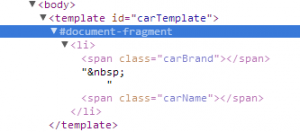
\includegraphics[height=3.0cm]{images/document_fragment.png}
\caption[
Visualisierung des DOM eines inaktiven Templates, Urldate: 04.2014
\newline
\small\texttt{\url{http://www.prevent-default.com/wp-content/uploads/2013/04/document-fragment-300x132.png}}
]{Visualisierung des DOM eines inaktiven Templates}
\label{fig:3_inactive_Template_DOM}
\end{figure}

In Abbildung \ref{fig:3_inactive_Template_DOM} auf Seite \pageref{fig:3_inactive_Template_DOM} wird gezeigt, dass das Template ein Dokument-Fragment ist. Dies bedeutet, dass es ein eigenständiges Dokument ist und unabhängig vom ursprünglichen Dokument existiert. Folglich bedeutet dies, dass sämtliche \lstinline|<script>, <form>, <img>, |-Tags etc. nicht verwendet werden können.

\begin{lstlisting}[language=JavaScript, caption={Verwendung des Templates \ref{lst:3_Templates} auf Seite \pageref{lst:3_Templates}}, label={lst:3_Templates_Verwendung}, escapeinside={@}{@}]
@\label{lst:3_Templates_Verwendung_1}@var template = document.getElementById('carTemplate');
template.content.querySelector(".carBrand").length; // length ist 1

@\label{lst:3_Templates_Verwendung_2}@var car = template.content.cloneNode(true);
car.querySelector(".carBrand").innerHTML = "Seat";
car.querySelector(".carName").innerHTML = "Ibiza";

@\label{lst:3_Templates_Verwendung_3}@document.getElementById("carList").appendChild(car);
\end{lstlisting}

Code-Beispiel \ref{lst:3_Templates_Verwendung} auf Seite \pageref{lst:3_Templates_Verwendung} basiert auf dem in Code-Beispiel \ref{lst:3_Templates} auf Seite \pageref{lst:3_Templates} definierten Template. Zu Beginn wird sich in Zeile \ref{lst:3_Templates_Verwendung_1} des Code-Beispiels \ref{lst:3_Templates_Verwendung} das bereits definierte Template in die Variable \lstinline|template| geholt. Daraufhin wird der gesamte Knoten in Zeile \ref{lst:3_Templates_Verwendung_2} mit Hilfe einer \lstinline|deep-copy| geklont und folglich mit Daten befüllt. Damit das mit Daten befüllte Listenelement auch sichtbar wird, wird es in Zeile \ref{lst:3_Templates_Verwendung_3} in das aktive DOM eingefügt.
